\chapter{Single Scenario Classification, KFold Validation}

Starting with fitting randomly the classifiers, there are some statistics of the data used for the first test: \\
 {\def\arraystretch{1.3} 
 \begin{table}[H] 
\centering 
\begin{tabular}{|l|l|l|} 
\hline 
  &count train  &count test  \\ \hline
messenger  &249  &100  \\ \hline
telegram  &244  &106  \\ \hline
whatsapp  &243  &107  \\ \hline
original  &243  &107  \\ \hline
\end{tabular} 
\end{table} }
\section{Logistic regression results:} 
Confusion matrix with number of sample and with normalization:
 {\def\arraystretch{1.3} 
 \begin{table}[H] 
\centering 
\begin{tabular}{|l|l|l|l|l|} 
\hline 
  &messenger  &telegram  &whatsapp  &original  \\ \hline
messenger  &100  &0  &0  &0  \\ \hline
telegram  &0  &106  &0  &0  \\ \hline
whatsapp  &0  &0  &103  &4  \\ \hline
original  &0  &0  &0  &107  \\ \hline
\end{tabular} 
\end{table} }

 \begin{figure}[H] 
\centering 
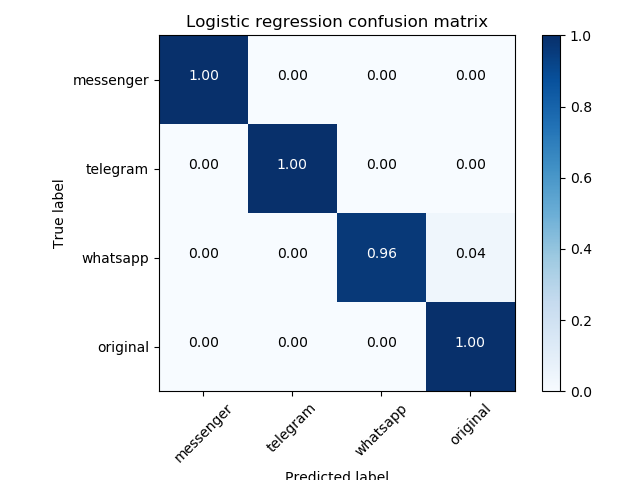
\includegraphics[scale=.6]{images/lr_initial.png} 
\caption{logistic regression} 
\end{figure} 


Result of the KFold validation with 10 bins:
 {\def\arraystretch{1.3} 
 \begin{table}[H] 
\centering 
\begin{tabular}{|l |l |l |l |l |l |l |l |l |l |}  
\hline 
0.9796&
0.9898&
1.0000&
1.0000&
1.0000&
0.9898&
0.9898&
1.0000&
0.9898&
1.0000\\ \hline  

\end{tabular} 
\end{table} }

The mean is : 0.993878\section{Linear Support Vector Machine results:}Confusion matrix with number of sample and with normalization:
 {\def\arraystretch{1.3} 
 \begin{table}[H] 
\centering 
\begin{tabular}{|l|l|l|l|l|} 
\hline 
  &messenger  &telegram  &whatsapp  &original  \\ \hline
messenger  &100  &0  &0  &0  \\ \hline
telegram  &0  &106  &0  &0  \\ \hline
whatsapp  &0  &0  &103  &4  \\ \hline
original  &0  &0  &0  &107  \\ \hline
\end{tabular} 
\end{table} }

 \begin{figure}[H] 
\centering 
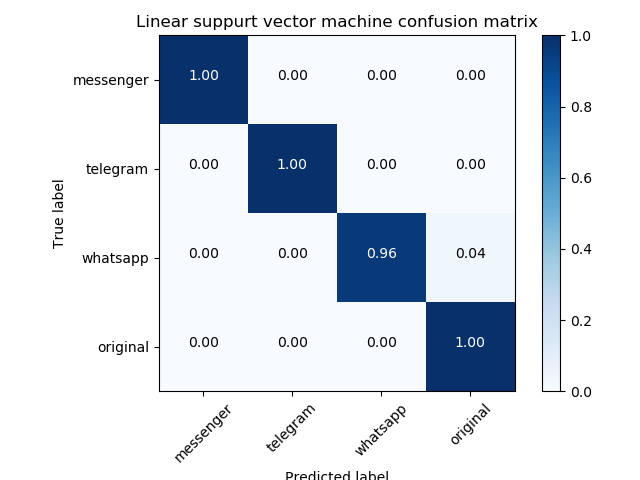
\includegraphics[scale=.6]{images/lsvm_initial.png} 
\caption{linear SVM} 
\end{figure} 


Result of the KFold validation with 10 bins:
 {\def\arraystretch{1.3} 
 \begin{table}[H] 
\centering 
\begin{tabular}{|l |l |l |l |l |l |l |l |l |l |}  
\hline 
0.9898&
0.9898&
1.0000&
1.0000&
1.0000&
0.9796&
0.9898&
1.0000&
0.9898&
1.0000\\ \hline  

\end{tabular} 
\end{table} }

The mean is : 0.993878\section{Random forest results:}Confusion matrix with number of sample and with normalization:
 {\def\arraystretch{1.3} 
 \begin{table}[H] 
\centering 
\begin{tabular}{|l|l|l|l|l|} 
\hline 
  &messenger  &telegram  &whatsapp  &original  \\ \hline
messenger  &100  &0  &0  &0  \\ \hline
telegram  &0  &106  &0  &0  \\ \hline
whatsapp  &0  &0  &103  &4  \\ \hline
original  &0  &0  &0  &107  \\ \hline
\end{tabular} 
\end{table} }

 \begin{figure}[H] 
\centering 
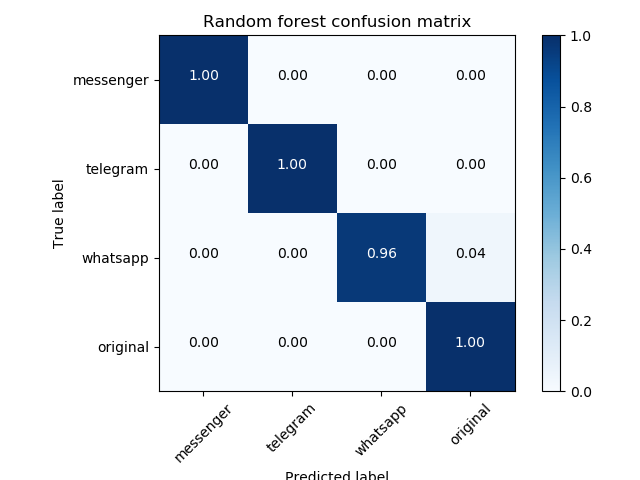
\includegraphics[scale=.6]{images/rf_initial.png} 
\caption{random forest} 
\end{figure} 


Result of the KFold validation with 10 bins:
 {\def\arraystretch{1.3} 
 \begin{table}[H] 
\centering 
\begin{tabular}{|l |l |l |l |l |l |l |l |l |l |}  
\hline 
1.0000&
0.9898&
1.0000&
1.0000&
1.0000&
0.9796&
0.9898&
1.0000&
0.9898&
0.9897\\ \hline  

\end{tabular} 
\end{table} }

The mean is : 0.993867

\chapter{Single Scenario Classification, Circularly Validation}

Here was used the same dataset as before but the training used a 0.3 of the dataset, and it is shifted circulary to cover all the dataset.Here is the table of all steps calculated \\
\begin{longtable} 
{|l |l |l |l |} 
\hline 
step  &logistic  &linear SVM  &random fo.  \\ \hline
0  &0.989179818268771  &0.9861800141743444  &0.9901213241201993  \\ \hline
1  &0.9848642886352729  &0.989179818268771  &0.9901086744322249  \\ \hline
2  &0.9859958494970797  &0.989179818268771  &0.992039295392954  \\ \hline
3  &0.9840239043824701  &0.989179818268771  &0.9879411617983916  \\ \hline
4  &0.9838346881813623  &0.989179818268771  &0.9878321961314647  \\ \hline
5  &0.9850775862706985  &0.9888435941925785  &0.9929795918367347  \\ \hline
6  &0.9849757394589151  &0.9899004065040651  &0.989900983984118  \\ \hline
7  &0.9869068386254386  &0.9899004065040651  &0.99103468547913  \\ \hline
8  &0.9859149679167976  &0.9899004065040651  &0.990969961616947  \\ \hline
9  &0.9826572092251535  &0.9861966137690223  &0.9817251354156551  \\ \hline
10  &0.9847290722474007  &0.9870545842786601  &0.9827326856656295  \\ \hline
11  &0.9837185571115683  &0.9857771334299855  &0.9846840787373938  \\ \hline
12  &0.9838354913678619  &0.9859658778205833  &0.9846840787373938  \\ \hline
13  &0.9813181579293129  &0.9861166500498505  &0.9807610095111248  \\ \hline
14  &0.9813181579293129  &0.9853611471537412  &0.9787703014260097  \\ \hline
15  &0.9831900496861925  &0.9862857095347368  &0.980725773647614  \\ \hline
16  &0.9841168266469769  &0.9862857095347368  &0.9808059618649602  \\ \hline
17  &0.9822572998070824  &0.9822572998070824  &0.9760144649257553  \\ \hline
18  &0.9821251322105606  &0.9822572998070824  &0.97795683313976  \\ \hline
19  &0.9820101172758178  &0.982107843137255  &0.9750549818320903  \\ \hline
20  &0.9820101172758178  &0.9826435137223949  &0.9769817171132961  \\ \hline
21  &0.9820101172758178  &0.9822440033492588  &0.9769817171132961  \\ \hline
22  &0.9820101172758178  &0.9819674282059272  &0.9769817171132961  \\ \hline
23  &0.9789859263543474  &0.9826435137223949  &0.9734258819806992  \\ \hline
24  &0.9789859263543474  &0.9844528594528594  &0.9734258819806992  \\ \hline
25  &0.9790240688968155  &0.9835470085470086  &0.9734258819806992  \\ \hline
26  &0.978963179539905  &0.9808615772912023  &0.9734258819806992  \\ \hline
27  &0.981011696187139  &0.9881608339538348  &0.981094861660079  \\ \hline
28  &0.9809466587092924  &0.9880438882784184  &0.981094861660079  \\ \hline
29  &0.978957428886153  &0.9869016393442622  &0.981094861660079  \\ \hline
30  &0.9771308523409363  &0.9880438882784184  &0.981094861660079  \\ \hline
31  &0.9839638554216867  &0.9889326989562411  &0.981094861660079  \\ \hline
32  &0.9821736011477762  &0.9839576074332173  &0.974576923076923  \\ \hline
33  &0.9632234670976825  &0.963381121890158  &0.9618357875948238  \\ \hline
34  &0.955915762290795  &0.9604524917457968  &0.9523383383383384  \\ \hline
35  &0.9558080031175651  &0.9615025224051383  &0.9332107165025093  \\ \hline
36  &0.9537713472485769  &0.9616828738173668  &0.9342712270274949  \\ \hline
37  &0.9567246849068246  &0.9705229237156167  &0.941807112194959  \\ \hline
38  &0.9624805441127516  &0.9689582071471836  &0.941807112194959  \\ \hline
39  &0.9656916766799837  &0.9754108565737052  &0.9426760297719203  \\ \hline
40  &0.9645393196105017  &0.9744245524296675  &0.9426760297719203  \\ \hline
41  &0.9674626293689195  &0.9725627105089125  &0.9426760297719203  \\ \hline
42  &0.9654192933722927  &0.970744883788362  &0.9435515300577979  \\ \hline
43  &0.9695591349062311  &0.9723367392625123  &0.9638905905957089  \\ \hline
44  &0.9684887580521552  &0.9724221573471613  &0.9735226067675696  \\ \hline
45  &0.968972132612202  &0.9742295202245372  &0.9713033424446343  \\ \hline
46  &0.9682197824252712  &0.9742295202245372  &0.9735226067675696  \\ \hline
47  &0.9693788613812181  &0.9731363489522036  &0.9724089271961905  \\ \hline
48  &0.9668187320808225  &0.9683336860555347  &0.9713033424446343  \\ \hline
49  &0.9642240738507779  &0.9642997792344016  &0.9631028529724224  \\ \hline
50  &0.9629520363275152  &0.9642997792344016  &0.9641429955913738  \\ \hline
51  &0.9631771897864273  &0.9642997792344016  &0.9609153080205712  \\ \hline
52  &0.9643385011275081  &0.9642997792344016  &0.9651904231493449  \\ \hline
53  &0.9738195798137318  &0.9726644779063561  &0.9702353383569476  \\ \hline
54  &0.9782388663967612  &0.9752631578947368  &0.9778754788737738  \\ \hline
55  &0.9782388663967612  &0.9695209703947368  &0.9778754788737738  \\ \hline
56  &0.9782388663967612  &0.9713281539030707  &0.9800443458980044  \\ \hline
57  &0.9789586940956656  &0.9714048901782014  &0.9789560728306903  \\ \hline
58  &0.9808488835137682  &0.9750631313131313  &0.980188679245283  \\ \hline
59  &0.9809913155949741  &0.9854702263238849  &0.9790973762010348  \\ \hline
60  &0.9820075757575757  &0.9808654423423285  &0.9800443458980044  \\ \hline
61  &0.9820075757575757  &0.9820075757575757  &0.9800443458980044  \\ \hline
62  &0.9820075757575757  &0.9820075757575757  &0.9780137313157126  \\ \hline
63  &1.0  &1.0  &0.9989837398373984  \\ \hline
64  &0.9949551291586097  &0.9939669421487604  &0.9858662941153005  \\ \hline
65  &0.9901960784313726  &0.9892578125  &0.9831053292616855  \\ \hline
66  &0.9901960784313726  &0.9892578125  &0.9898912530352956  \\ \hline
67  &0.9901960784313726  &0.9892578125  &0.9920351473922903  \\ \hline
68  &0.9881717869333969  &0.9852417482429718  &0.986020872302839  \\ \hline
69  &0.9881717869333969  &0.9861800141743444  &0.9910744534968137  \\ \hline
\end{longtable} 
Average of all steps: 

 {\def\arraystretch{1.3} 
 \begin{table}[H] 
\centering 
\begin{tabular}{|l|l|l|} 
\hline 
logistic r.  &linear SVM  &random f.  \\ \hline
0.9777519138070937  &0.9801399772382293  &0.9746721183192149  \\ \hline
\end{tabular} 
\end{table} }
Confusion matrix estimated on overall tests: 

 \begin{figure}[H] 
\centering 
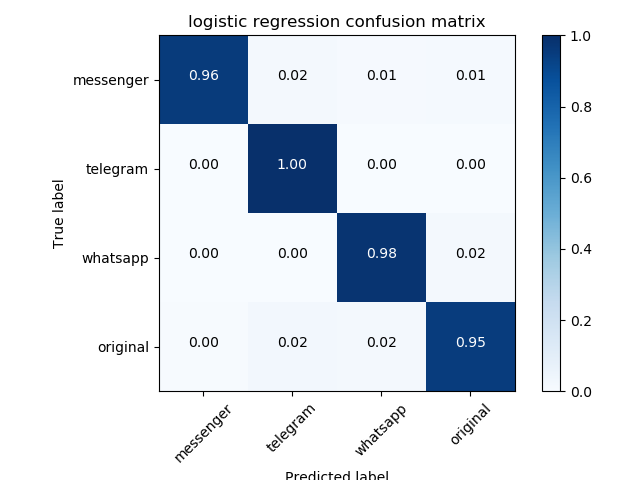
\includegraphics[scale=.6]{images/logistic_total.png} 
\caption{logistic regression} 
\end{figure} 

 \begin{figure}[H] 
\centering 
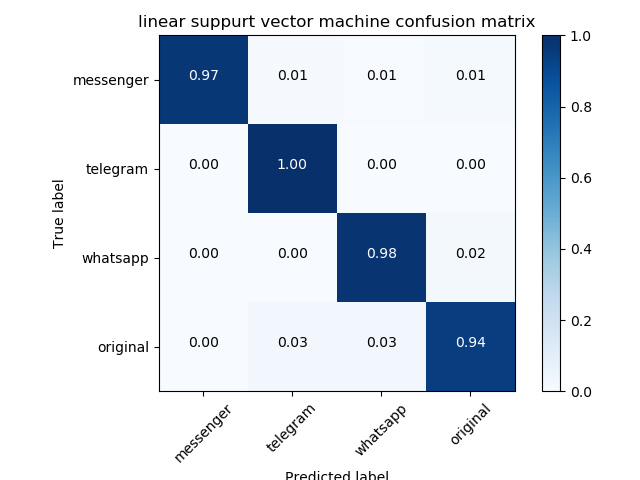
\includegraphics[scale=.6]{images/lsvm_total.png} 
\caption{linear SVM} 
\end{figure} 

 \begin{figure}[H] 
\centering 
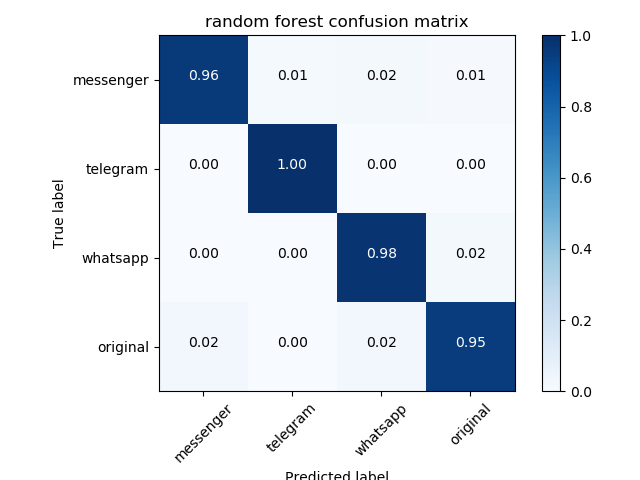
\includegraphics[scale=.6]{images/random_total.png} 
\caption{random forest} 
\end{figure} 
